%\begin{tcolorbox}
%Teilt eure Klassendiagramme bitte auf und baut \textbf{kein} einzelnes riesiges Diagramm.
%Getter und Setter Methoden müssen hier nicht modelliert werden.
%Sie sollten aber der klassischen Namenskonvention folgen, um die Nutzung in Sequenzdiagrammen zu ermöglichen.
%\\\\
%Auf jedes Diagramm folgt eine Tabelle, in der die Aufgabe \textbf{jeder} Klasse beschrieben wird.
%\end{tcolorbox}

\section{Backend}

\subsection{Backend Datenmodell}

\begin{figure}[h]
	\centering
	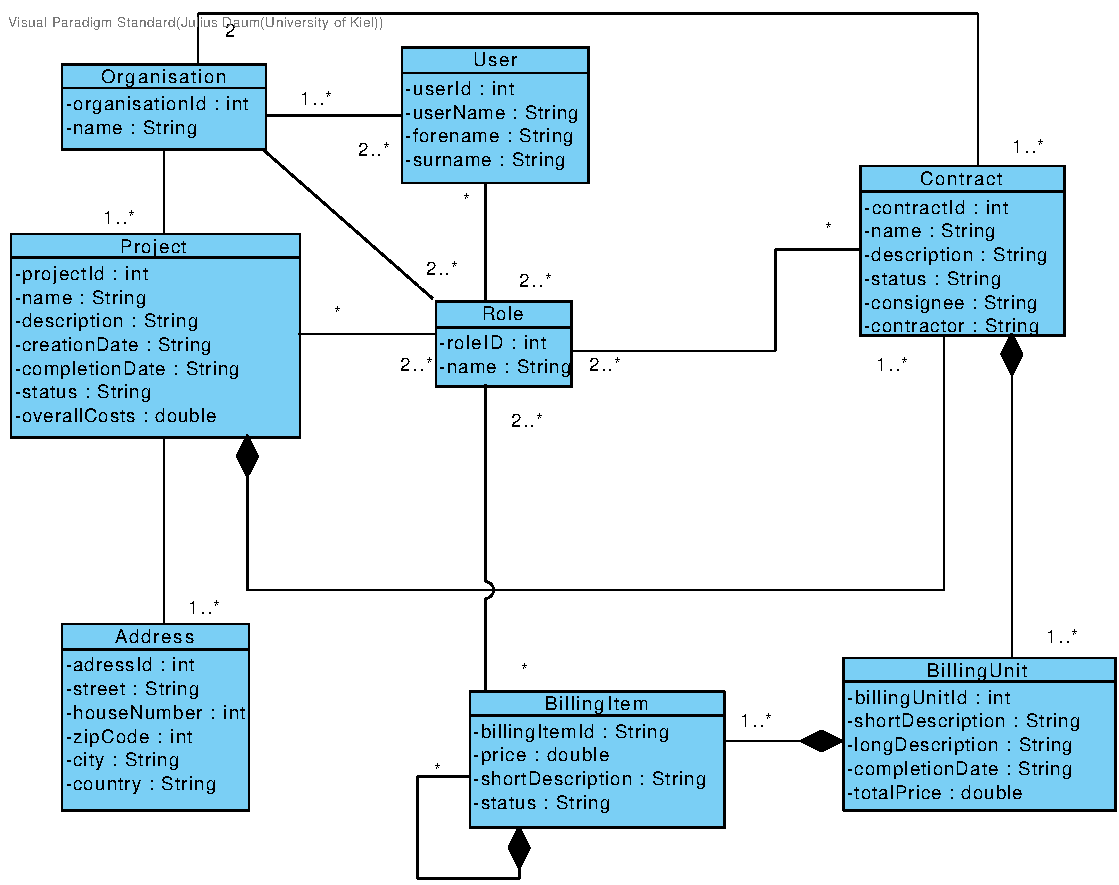
\includegraphics[width=15cm]{img/diagrams/class-diagram-backend.pdf}
	\caption{Klassendiagramm - Backend - Datenmodell}
	\label{fig:klassendiagramm-backend-model}
\end{figure}

\clearpage

\noindent
Dieses Klassendiagramm enthält die Entitäten der Datenbank, jede Klasse entspricht einer Entität. \\
Die Klassen \textbf{BillingItem}, \textbf{Contract}, \textbf{User}, \textbf{Organisation} und \textbf{Project} stehen jeweils mit mindestens 2 Instanzen der Klasse \textbf{Role} in Beziehung, da der \textbf{SysAdmin} Mitglied jeder Organisation ist und somit alle Projekte, User, Verträge und Leistungspositionen einsehen kann.
Zusätzlich existiert zu jeder Organisation mindestens ein \textbf{OrgAdmin}, der ebenfalls auf alle seiner Organisation zugeordneten Verträge, Projekte und Leistungspositionen zugreifen kann.
 
\begin{longtable}[h]{p{5cm} p{9cm}}
	\caption{Klassenbeschreibung - Backend - Datenmodell}
	\label{table:klassenbeschreibung-backend}
    \endlastfoot
	\multicolumn{2}{r}{{Weitergeführt auf der folgenden Seite}} \\
	\endfoot
	\endhead
	\rowcolor[HTML]{C0C0C0} 
	\textbf{Klassenname} & \textbf{Aufgabe} \\
    
	Address & Die Adresse des Projekts. \\
	
	\rowcolor[HTML]{E7E7E7} 
	BillingItem & Die Leistungsposition eines Vertrages. \\
	
	BillingUnit & Eine Gruppierung von Leistungspositionen. \\
	
	\rowcolor[HTML]{E7E7E7} 
	Contract & Ein Vertrag, welcher zwischen zwei Parteien geschlossen wird. \\
	
	Organisation & Eine Gruppierung von \textbf{User}n. \\
	
	\rowcolor[HTML]{E7E7E7} 
	Project & Ein Projekt mindestens einer Organisation, welches mehrere Verträge enhalten kann. \\
	
	Role & Nutzerrollen mit verschiedenen Rechten. \\

	\rowcolor[HTML]{E7E7E7}
	User & Mitarbeiter mindestens einer Organisation.
\end{longtable}

\subsection{Backend Datenverarbeitung}

\begin{figure}[H]
	\centering
	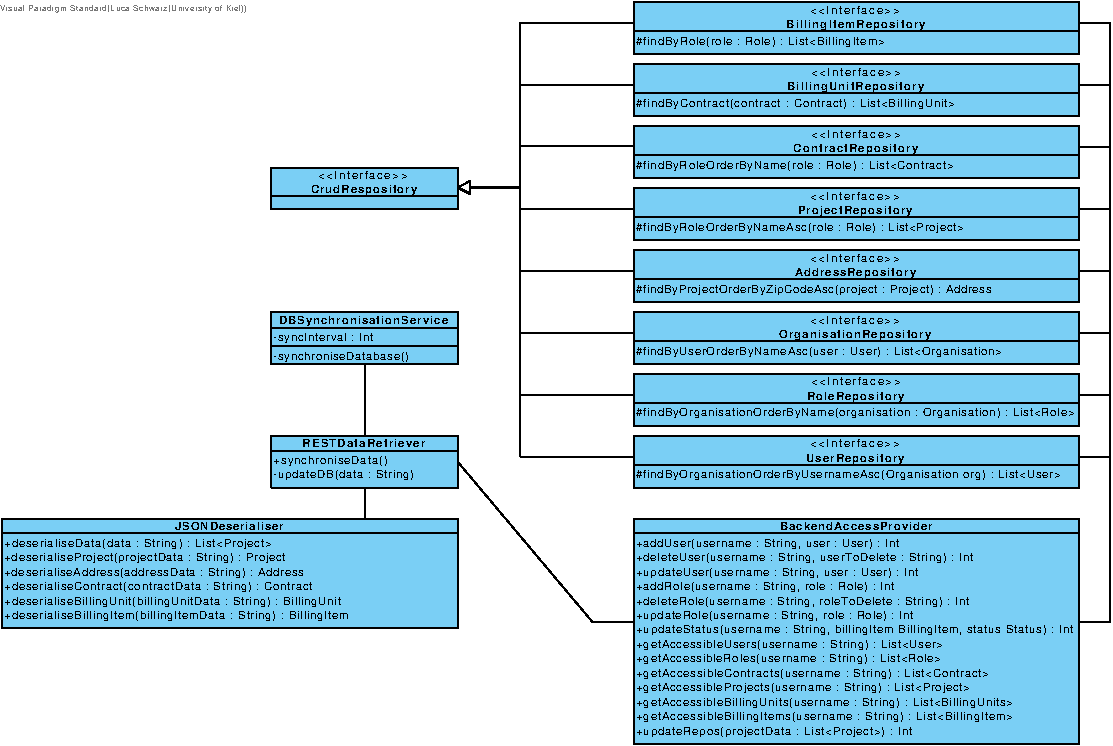
\includegraphics[width=\linewidth]{img/diagrams/Backend.pdf}
	\caption{Klassendiagramm - Backend - Datenverarbeitung}
	\label{fig:klassendiagramm-backend-data}
\end{figure}

\clearpage

\begin{center}
\begin{longtable}[h]{p{5cm} p{9cm}}
	\caption{Klassenbeschreibung - Backend - Datenverarbeitung}
	\label{table:klassenbeschreibung-backend-data}
	\endlastfoot
	\multicolumn{2}{r}{{Weitergeführt auf der folgenden Seite}} \\
	\endfoot
	\endhead
	\rowcolor[HTML]{C0C0C0} 
	\textbf{Klassenname} & \textbf{Aufgabe} \\
    CrudRepository & Teil des Spring Frameworks. Wird hier genutzt, um die Datenbank in Form von erbenden Repositories darzustellen. \\
	\rowcolor[HTML]{E7E7E7} 
	*Repository & Verwaltet die jeweilige Datenmodellklasse. Bietet spezielle Zugriffsfunktionen für eine einfachere Nutzung. \\
	BackendAccessProvider & Bietet die eigentliche Funktionalität des Backends innerhalb der Server-Applikation an. Über diese Klasse wird der gesicherte Zugriff auf die gespeicherten Daten sichergestellt und die 
    einzelnen Daten-Repositories werden vor dem Nutzer verborgen. Alle Methoden verlangen einen Nutzernamen als Parameter, um festzustellen, welche Daten zurückgegeben werden dürfen. Dafür werden intern die Rollen verwendet.
    So soll ein Nutzer z.B. nur Zugriff auf Verträge bekommen, für die er auch über eine entsprechende Rolle verfügt. Ansonsten werden leere Listen und auch Fehlercodes zurückgegeben, welche dann z.B. vom Frontend
    entsprechend verarbeitet werden können. Die Controller-Klassen des Frontends haben folglich Zugriff auf den \textbf{BackendAccessProvider}. \\
	\rowcolor[HTML]{E7E7E7} 
	DBSynchronisationService & Dienst, welcher nach einem Zeitintervall eine Synchronisation zwischen der Datenbank von adesso und der lokalen veranlasst. 
	Die eigentliche Synchronisation führt die Klasse \textbf{RESTDataRetriever} durch. \\
    RESTDataRetriever & Fragt die Daten über die \textbf{REST-API} von adesso ab und deserialisiert diese anschlie{\ss}end. Die so erhaltenen Klassen werden abschließend in die Datenbank über den \textbf{BackendAccessProvider} eingepflegt. \\
	\rowcolor[HTML]{E7E7E7} 
    JSONDeserialiser & Konvertiert \textbf{JSON}-Strings in die entsprechenden Modellklassen. Dies findet Verwendung, wenn die Daten über die \textbf{REST-API} von adesso abgefragt werden. \\
\end{longtable}
\end{center}

\clearpage

\section{Web}

\begin{figure}[h]
	\centering
	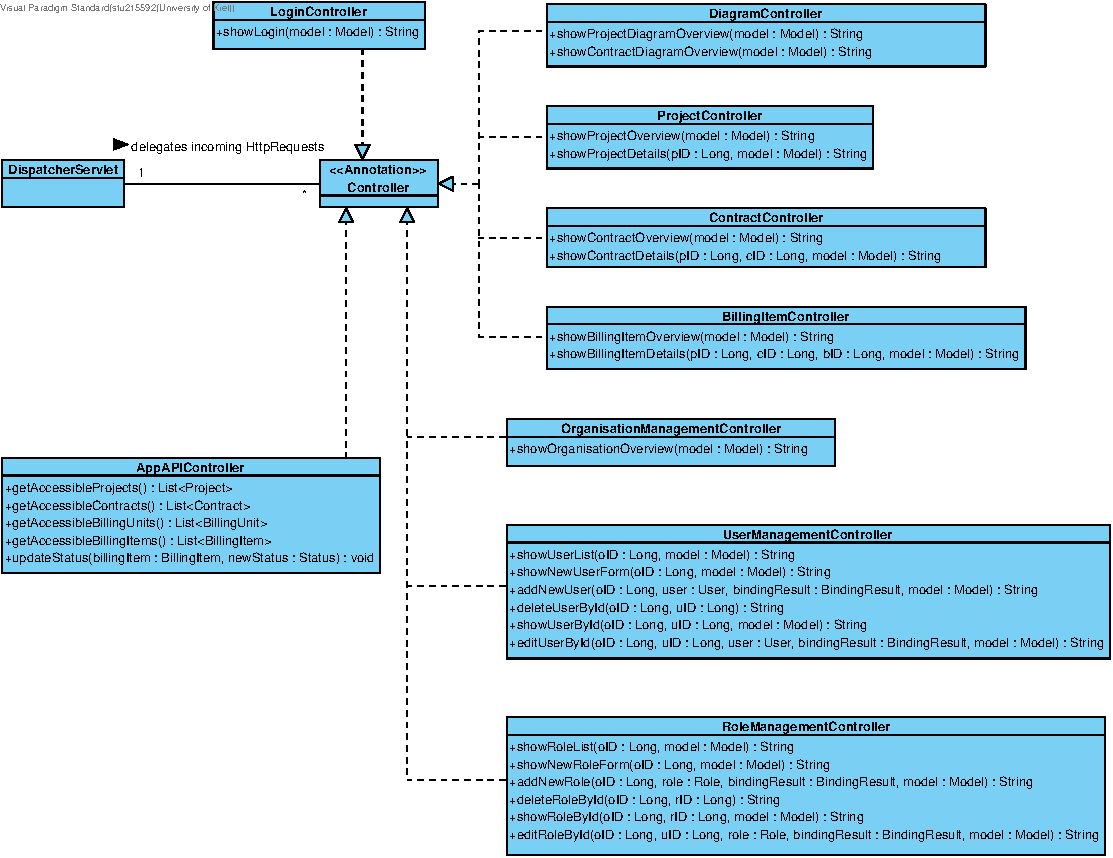
\includegraphics[width=\linewidth]{img/diagrams/Frontend Classes.pdf}
	\caption{Klassendiagramm - Web}
	\label{fig:klassendiagramm-web}
\end{figure}

\noindent
\textbf{Controller} verarbeiten HTTP-Requests zu bestimmten Pfaden.
Die Pfade werden von je einem \textbf{Controller} nach Gebiet gruppiert verarbeitet.
Diese werden in der folgenden Tabelle unter Aufgabe aufgeführt.
Die Identifikationsnummern oID (Organisation), uID (Nutzer), rID (Rolle), pID (Projekt), cID (Vertrag) und bID (Leistungsposition) sind in einigen Pfaden direkt integriert.\\

\begin{longtable}[h]{p{5.3cm} p{8.7cm}}
	\caption{Klassenbeschreibung - Web}
	\label{table:klassenbeschreibung-web}
	\endlastfoot
	\multicolumn{2}{r}{{Weitergeführt auf der folgenden Seite}} \\
	\endfoot
	\endhead
	\rowcolor[HTML]{C0C0C0} 
	\textbf{Klassenname} & \textbf{Aufgabe} \\
    
	DispatcherServlet & Teil des Spring Frameworks, leitet die HTTP-Requests an den jeweils zuständigen \textbf{Controller} weiter. \\
	
	\rowcolor[HTML]{E7E7E7} 
	LoginController & /login $\rightarrow$ Login-Seite \\
	
	OrganisationManagementController & /organisation\_overview $\rightarrow$ Management von Organisationen und deren \textbf{OrgAdmin}s, nur der \textbf{SysAdmin} hat hierauf Zugriff \\
	
	\rowcolor[HTML]{E7E7E7} 
	UserManagementController & /organisation/\{oID\}/user\_management $\rightarrow$ Management der \textbf{WebUser} einer Organisation \newline\newline
	/organisation/\{oID\}/user\_management/user\_new $\rightarrow$ Hinzufügen eines \textbf{WebUser}s zu einer Organisation \newline\newline
	/organisation/\{oID\}/user\_management/user/\{uID\} /user\_edit $\rightarrow$ Bearbeiten eines \textbf{WebUser}s einer Organisation \\
	
	RoleManagementController & /organisation/\{oID\}/role\_management $\rightarrow$ Management der Rollen einer Organisation \newline\newline
	/organisation/\{oID\}/role\_management/role\_new $\rightarrow$ Hinzufügen einer Rolle zu einer Organisation \newline\newline
	/organisation/\{oID\}/role\_management/role/\{rID\} /role\_edit $\rightarrow$ Bearbeiten einer Rolle einer Organisation \\
	
	\rowcolor[HTML]{E7E7E7} 
	ProjectController & /project\_overview $\rightarrow$ Zeigt alle Projekte an, für welche der \textbf{WebUser} die nötigen Berechtigungen hat \newline\newline
	/project/\{pID\}/show $\rightarrow$ Zeigt die Verträge des Projekts an, für welche der \textbf{WebUser} die nötigen Berechtigungen hat \\
	
	ContractController & /contract\_overview $\rightarrow$ Zeigt alle Verträge an, für welche der \textbf{WebUser} die nötigen Berechtigungen hat \newline\newline
	/project/\{pID\}/contract/\{cID\}/show $\rightarrow$ Zeigt die Leistungspositionen des Vertrags an, für welche der \textbf{WebUser} die nötigen Berechtigungen hat \\
	
	\rowcolor[HTML]{E7E7E7} 
	BillingItemController & /billing\_item\_overview $\rightarrow$ Zeigt alle Leistungspositionen an, für welche der \textbf{WebUser} die nötigen Berechtigungen hat \newline\newline
	/project/\{pID\}/contract/\{cID\}/billing\_item/\{bID\}/show $\rightarrow$ Zeigt Details zur Leistungsposition an, falls der \textbf{WebUser} die nötigen Berechtigungen hat \\
	
	DiagramController & /project\_diagram\_overview $\rightarrow$ Zeigt alle Diagramme zu Projekten an, für welche der \textbf{WebUser} die nötigen Berechtigungen hat \newline\newline
	/contract\_diagram\_overview $\rightarrow$ Zeigt alle Diagramme zu Verträgen an, für welche der \textbf{WebUser} die nötigen Berechtigungen hat
\end{longtable}

\clearpage

\section{App}

\begin{figure}[h]
	\centering
	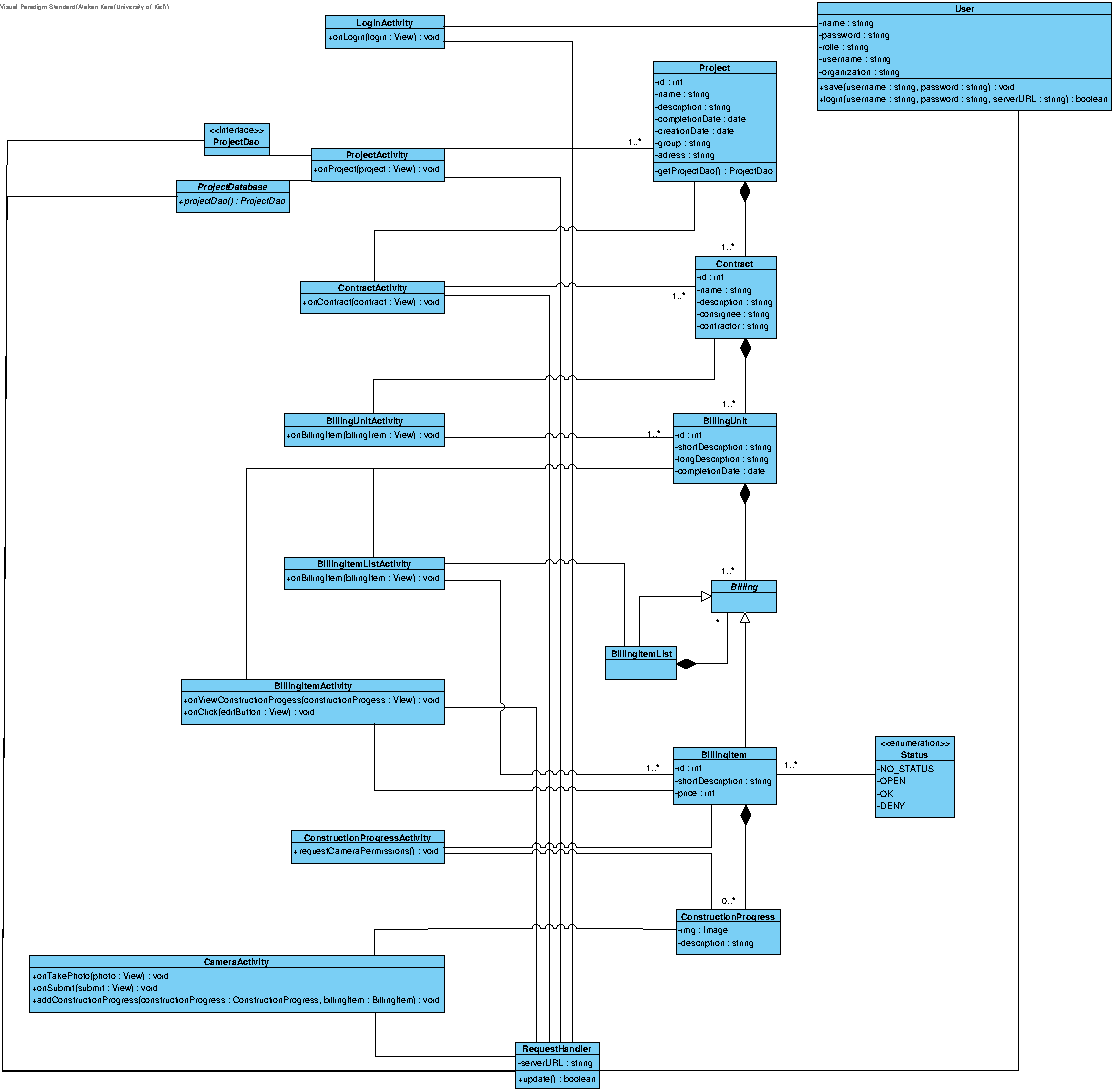
\includegraphics[width=\linewidth]{img/diagrams/Classdiagram-App.pdf}
	\caption{Klassendiagramm - App}
	\label{fig:klassendiagramm-a}
\end{figure}

\noindent
Alle Activity-Klassen enthalten neben den angegebenen auch die folgenden Methoden: onLogout(), onBack(), onCreate(), onStart(), onResume(), onPause(), onStop(), onRestart(), onDestroy().
Außerdem wird mittels der abstrakten Klasse Billing das Composite-Strukturmuster verwendet.\\

\clearpage

\begin{table}[h]
	\centering
	\begin{tabularx}{\textwidth}{X X}
		\rowcolor[HTML]{C0C0C0} 
		\textbf{Klassenname} & \textbf{Aufgabe} \\
		Project & Bauplan eines Projekts mit den jeweiligen Attributen.\\
		
		\rowcolor[HTML]{E7E7E7} 
		Contract & Bauplan eines Vertrages mit den jeweiligen Attributen. \\
		
		BillingUnit & Bauplan einer Leistungseinheit mit den jeweiligen Attributen. \\
		
		\rowcolor[HTML]{E7E7E7} 
		ConstructionProgress & Bauplan einer Baufortschritts-Klasse mit den jeweiligen Attributen. \\
		
		LoginActivity & Verwaltung des Login-Bildschirms. \\
		
		\rowcolor[HTML]{E7E7E7} 
		ProjectActivity & Verwaltung des Projekt-Bildschirms. \\
		
		ContractActivity & Verwaltung des Vertags-Bildschirms. \\
		
		\rowcolor[HTML]{E7E7E7} 
		BillingUnitActivity & Verwaltung des Leistungspositioneinheits-Bildschirms. \\
		
		BillingItemListActivity & Verwaltung des Leistunspositionlisten-Bildschirms. \\
		
		\rowcolor[HTML]{E7E7E7} 
		BillingItemActivity & Verwaltung des Leistunspositions-Bildschirms. \\
		
		ConstructionProgressActivity & Verwaltung des Baufortschritts-Bildschirms. \\
		
		\rowcolor[HTML]{E7E7E7} 
		CameraActivity & Verwaltung des Kamera-Bildschirms. \\
		
		RequestHandler & Verwaltung der Netzwerkanfragen aller Klassen. \\
		
		\rowcolor[HTML]{E7E7E7} 
		ProjectDao & Datenzugriffsobjekt mit Anfragen zur Interaktion mit der Projektdatenbank. \\
		
		ProjectDatabase & Room-Datenbank für Projekte. \\
		
		\rowcolor[HTML]{E7E7E7} 
		Status & Aufzählung, welche den Status modelliert.\\
	
		User & Nutzer der App. \\
		
		\rowcolor[HTML]{E7E7E7}
		Billing & Abstrakte Klasse, dient dem Composite-Strukturmuster. \\
		
		BillingItemList & Kompositum, welches \textbf{BillingItem}s enthält. \\
		
		\rowcolor[HTML]{E7E7E7}
		BillingItem & Blatt des Kompositums, Bauplan einer Leistungsposition mit den jeweiligen Attributen. \\
	\end{tabularx}
	\caption{Klassenbeschreibung - App}
	\label{table:klassenbeschreibung-a}
\end{table}
